\section{方案设计}

\subsection{技术路线}

\begin{frame}
    \frametitle{技术路线}

    \begin{itemize}
        \item 编程语言:Golang
        \item 密码学库:crypto/ecdsa, \texttt{github.com/tuneinsight/lattigo/v4}
        \item 数据库:SQLite3,及 \texttt{github.com/mattn/go-sqlite3}
    \end{itemize}

\end{frame}

\begin{frame}
    \frametitle{数据库设计}

    \begin{figure}[h]
        \centering
        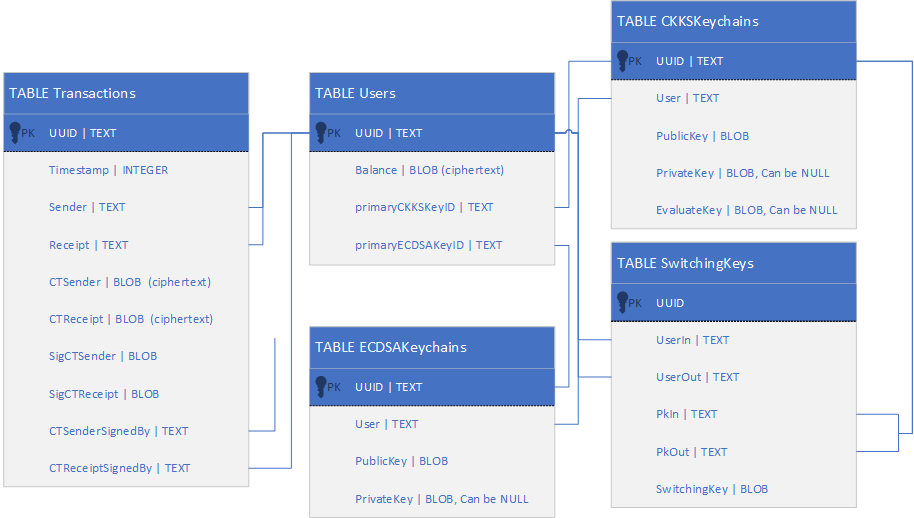
\includegraphics[width=0.8\linewidth]{figures/chimata-database-design.png}
        \caption{数据库设计抽象}
    \end{figure}

\end{frame}

\subsection{交易流程描述}

\begin{frame}
    \frametitle{交易流程 - 总体}

    \begin{figure}[h]
        \centering
        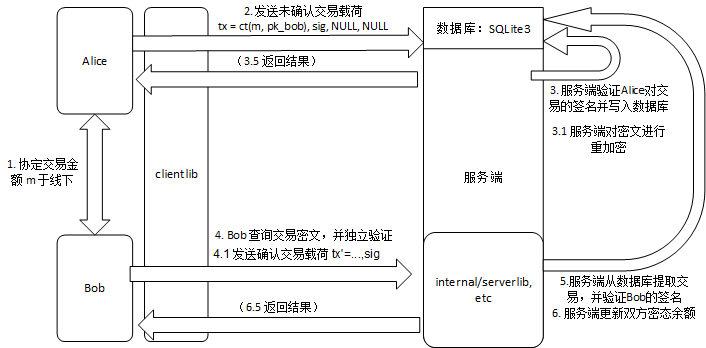
\includegraphics[width=0.75\linewidth]{figures/Tx-Abstract.png}
    \end{figure}

    此外方案代码也提供了一个以转出方公钥加密的交易发起的实现,和下文类似,仅无确认流程。这里不再赘述。
\end{frame}

\begin{frame}
    \frametitle{交易流程 - 转出方发起}

    \begin{itemize}
        \item Alice 与 Bob 协定交易金额 $m$
        \item Alice 通过以下调用方法,向服务端发送请求:
        \begin{itemize}
            \item 以用户 bob 和交易金额 $m$ 为参数调用 \texttt{alice.TransferByReceiptPK(bob, m)} 以生成需要提交的交易结构体 \newline 包括加密交易金额和对密文签名,生成交易载荷 $tx = \{NULL, NULL, ct_b, sig\}$
            \item 调用 \texttt{alice.CreateTransferJob(tx)} 和服务端进行网络交互 \newline 将交易载荷反序列化为 JSON,通过 http 发送到服务端接口 \texttt{(server)/transaction/create/byReceiptPK}
            
        \end{itemize}
    \end{itemize}

\end{frame}

\begin{frame}
    \frametitle{交易流程 - 服务端验证和重加密}

    \begin{itemize}
        \item 服务端接收到交易发起请求,调用方法 \texttt{HandlerTransactionCreateByReceiptPK}
        \begin{itemize}
            \item 使用 Alice 的 ECDSA 公钥对交易密文的签名进行验证
            \item 使用 $swk_{Bob \rightarrow Alice}$ 进行重加密
            \item 写入数据库,向 Alice 返回结果,包括分配的 uuid 等 
        \end{itemize}
        \item 若服务端任何一处出现问题,则返回非 200 代码,包含具体错误于键值对 \texttt{"error": (actual error message)} 中。
    \end{itemize}

\end{frame}

\begin{frame}
    \frametitle{交易流程 - 转入方确认和服务端更新账户}

    \begin{itemize}
        \item Bob 可以以 uuid 向服务端查询交易,获得交易信息 \texttt{txNew},并验证是否金额是否正确
        \item Bob 对交易中以 Alice 的公钥加密的密文进行签名,并提交给服务器
        \begin{itemize}
            \item 调用 \texttt{bob.AcceptTransactionByTransaction(txNew)} 进行签名的生成
            \item 调用 \texttt{bob.CreateConfirmTransactionTask(txNew)} 将签名后的交易发送给服务端接口 \texttt{(server)/transaction/confirm},等待回应
        \end{itemize}
        \item 服务端接收到交易接受请求,进行验证;
        \item 服务端更新交易双方密文余额,并写入数据库
        \begin{itemize}
            \item 即:对转出方密态余额减去交易金额,对转入方密态余额加上交易金额。
        \end{itemize}
    \end{itemize}

\end{frame}

\subsection{方案相关分析}

\begin{frame}
    \frametitle{分析}

    \begin{itemize}
        \item 隐私性:由 CKKS 方案保证
        \begin{itemize}
            \item R-LWE 问题:归约至 SVP 问题,NP-Hard,and post-quantum
        \end{itemize}
        \item 不可伪造性:由 ECDSA 签名方案保证:
        \begin{itemize}
            \item 交易双方对密文摘要进行签名
            \item 伪造是困难的
        \end{itemize}
        \item 可交易性与正确性:由基于 R-LWE 假设的加密方案的相关性质保证
        \begin{itemize}
            \item 浮点数的同态性:保证了可以正确更新密态余额和计算手续费
            \item R-LWE 的密钥交换方法:正确性
        \end{itemize}
    \end{itemize}

\end{frame}
